\section{Dataset and Preprocessing}
\label{sec:data}

\subsection{METR-LA Dataset}
\label{subsec:dataset}

The experiments were conducted on the METR-LA dataset, which contains
traffic-speed measurements collected from 207 loop detectors located on the
Los Angeles County road network. Measurements are sampled every five minutes,
resulting in 34,272 timestamps covering the period from March 1 to June 27,
2012. Each sensor is associated with a single feature representing the
observed traffic speed.

The dataset can therefore be represented as a multivariate time series
$\mathbf{X} \in \mathbb{R}^{T \times N}$, where $T=34{,}272$ denotes the
number of timestamps and $N=207$ the number of traffic sensors. The spatial
relationships between sensors are represented by the graph provided with the
dataset. Its adjacency matrix $\mathbf{A} \in \mathbb{R}^{N \times N}$ is
directed and weighted and is later used by the graph-temporal model for
spatial message passing. A detailed description of the graph construction and
normalization is provided in Section~\ref{subsec:graph}.


\subsection{Exploratory Data Analysis}
\label{subsec:eda}

Before defining the preprocessing pipeline, an exploratory analysis was
performed to investigate the temporal structure, data quality, and variability
of the traffic measurements. The temporal index was found to be regularly
spaced, with no duplicated timestamps and no explicit NaN or infinite values
in the original data.

Particular attention was devoted to zero-valued measurements. Approximately
8.11\% of all observations are equal to zero, and zero values occur for all
207 sensors, although with considerably different frequencies across nodes.
More importantly, several timestamps contain simultaneous zero measurements
across the entire sensor network. The longest consecutive sequence consists
of 381 timestamps, corresponding to approximately 31 hours and 45 minutes
during which no sensor reports a positive traffic speed.

The temporal concentration of these measurements suggests that a substantial
fraction of the zero values represents unavailable or invalid sensor readings
rather than actual zero traffic speed. This behavior is illustrated in
Figure~\ref{fig:mean_speed_zero_comparison}. When zero values are included in the
network-wide average, several abrupt drops appear in correspondence with
periods in which a large number of sensors simultaneously report zero
measurements. After excluding zero-valued observations, these artificial
drops disappear and intervals in which the entire network is unavailable
appear as gaps in the time series.

This provides additional evidence that zero measurements should not be
interpreted directly as actual traffic speeds. Based on this analysis,
zero-valued measurements were therefore treated as missing observations in
the subsequent preprocessing pipeline.

\begin{figure}[htbp]
    \centering

    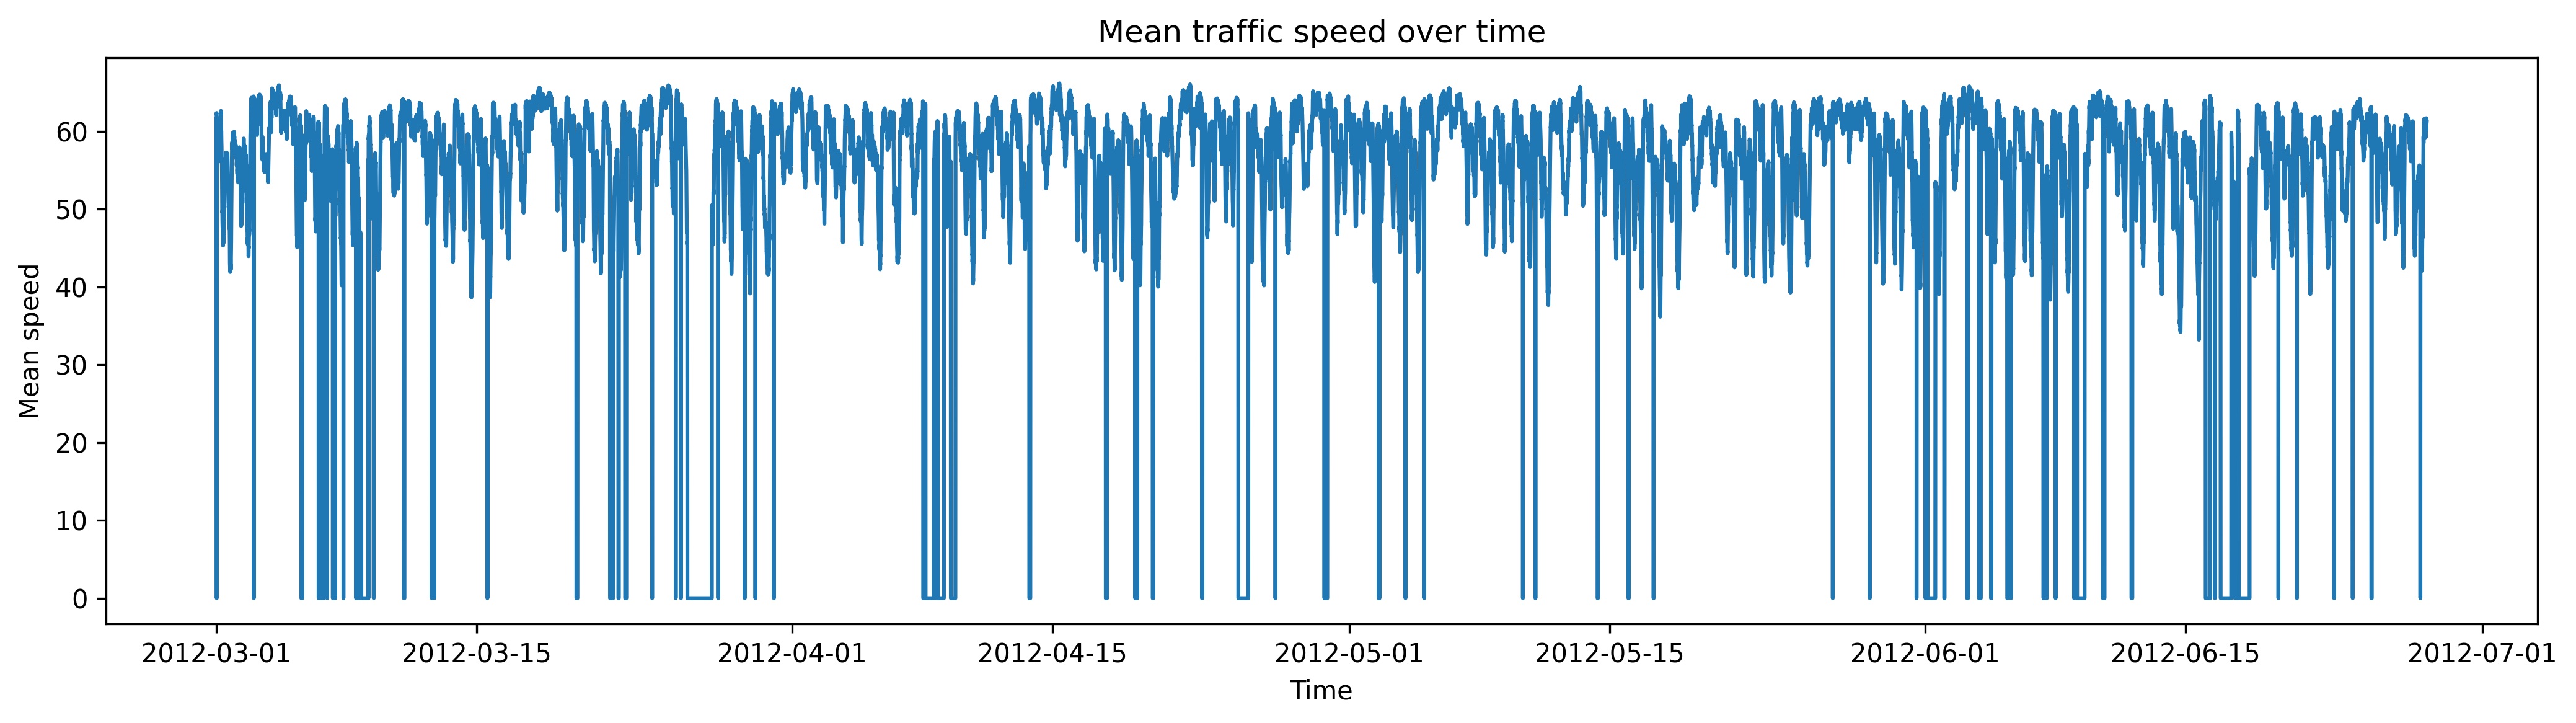
\includegraphics[width=\textwidth]{img/data_analysis/mean_speed_with_zeros}

    \vspace{0.3cm}

    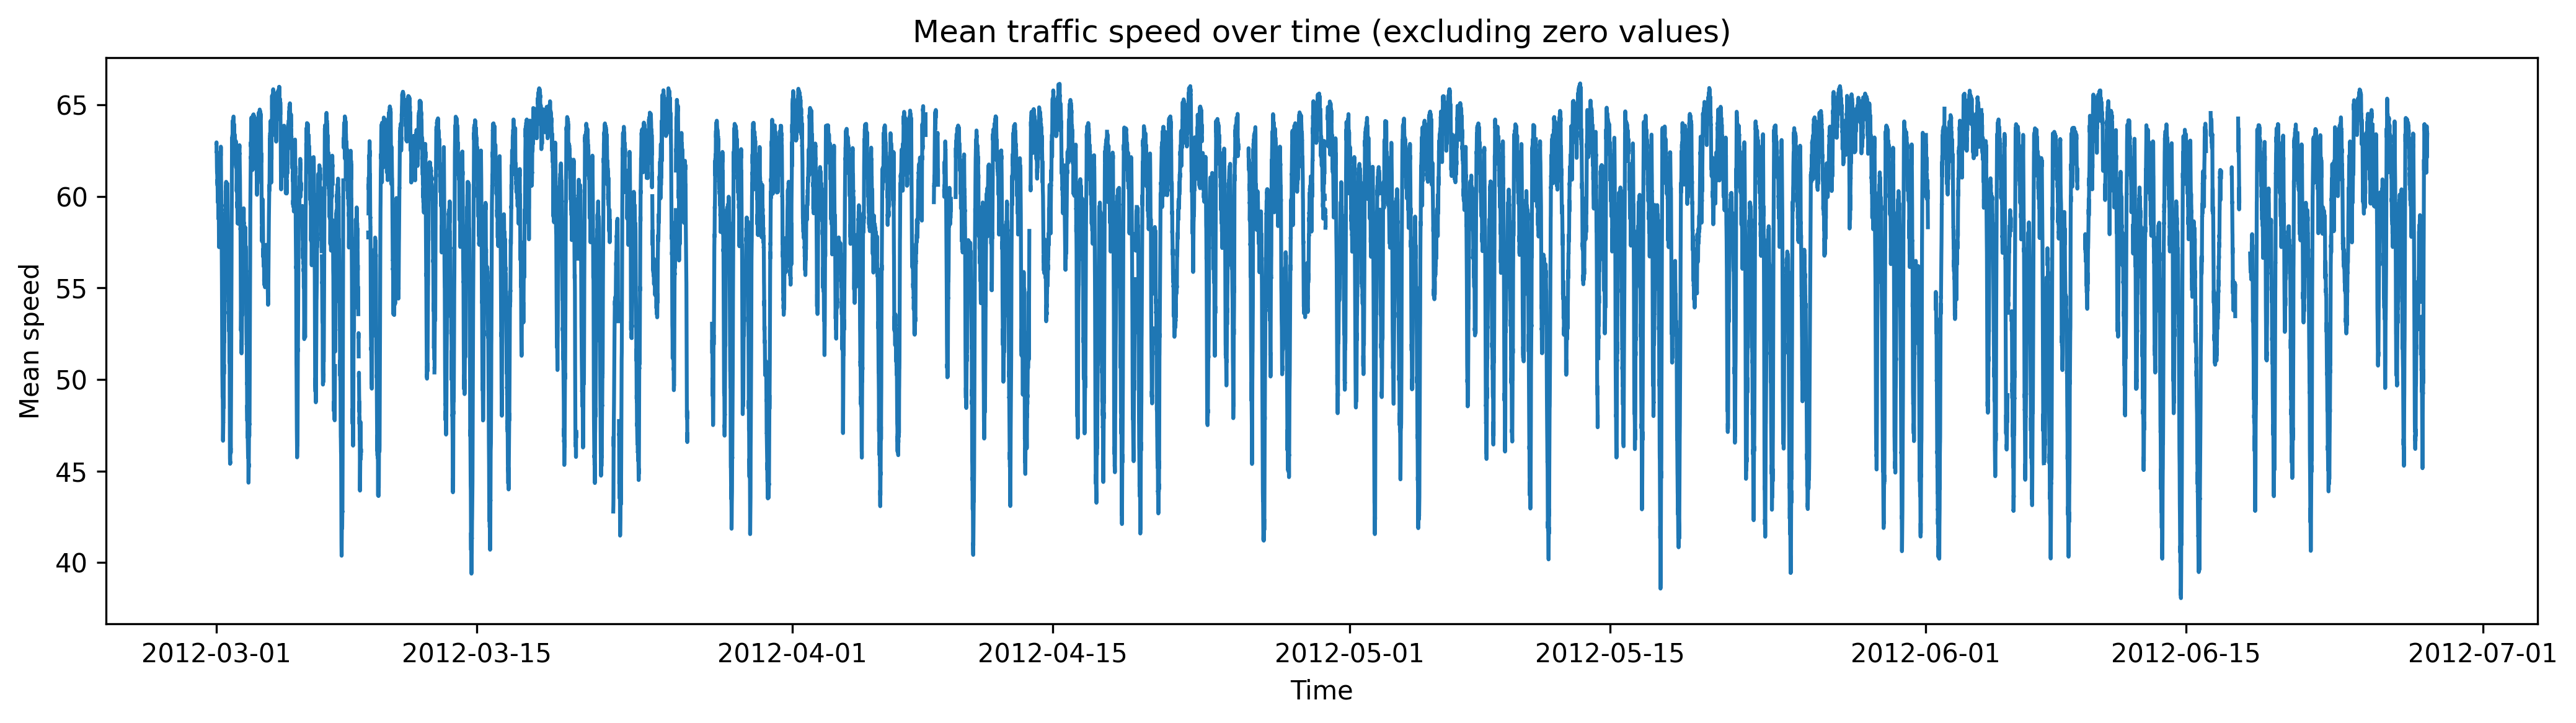
\includegraphics[width=\textwidth]{img/data_analysis/mean_speed_without_zeros}

    \caption{Mean traffic speed over time before (top) and after (bottom) excluding zero values.
    Removing zero-valued measurements eliminates the abrupt drops to zero while preserving the temporal traffic patterns.}
    \label{fig:mean_speed_zero_comparison}
\end{figure}


The valid traffic measurements also exhibit strong temporal structure.
Aggregating traffic speeds by hour of the day reveals a clear daily
seasonality, with average speeds decreasing during typical congestion periods
and increasing again during less congested hours. However, aggregating all
days together partially hides differences between working days and weekends.

Figure~\ref{fig:temporal_patterns} therefore compares the hourly traffic-speed
profiles obtained separately for weekdays and weekends. Weekdays exhibit more
pronounced reductions in average speed during the morning and especially
during the afternoon and evening, whereas weekends show a smoother profile
with generally higher speeds during the corresponding periods. The figure
therefore reveals a weekly component in addition to the daily seasonality.

These observations confirm that the traffic series contains meaningful
temporal dependencies at multiple time scales and motivate the use of a
temporal forecasting model in the subsequent experiments.

\begin{figure}[t]
    \centering
    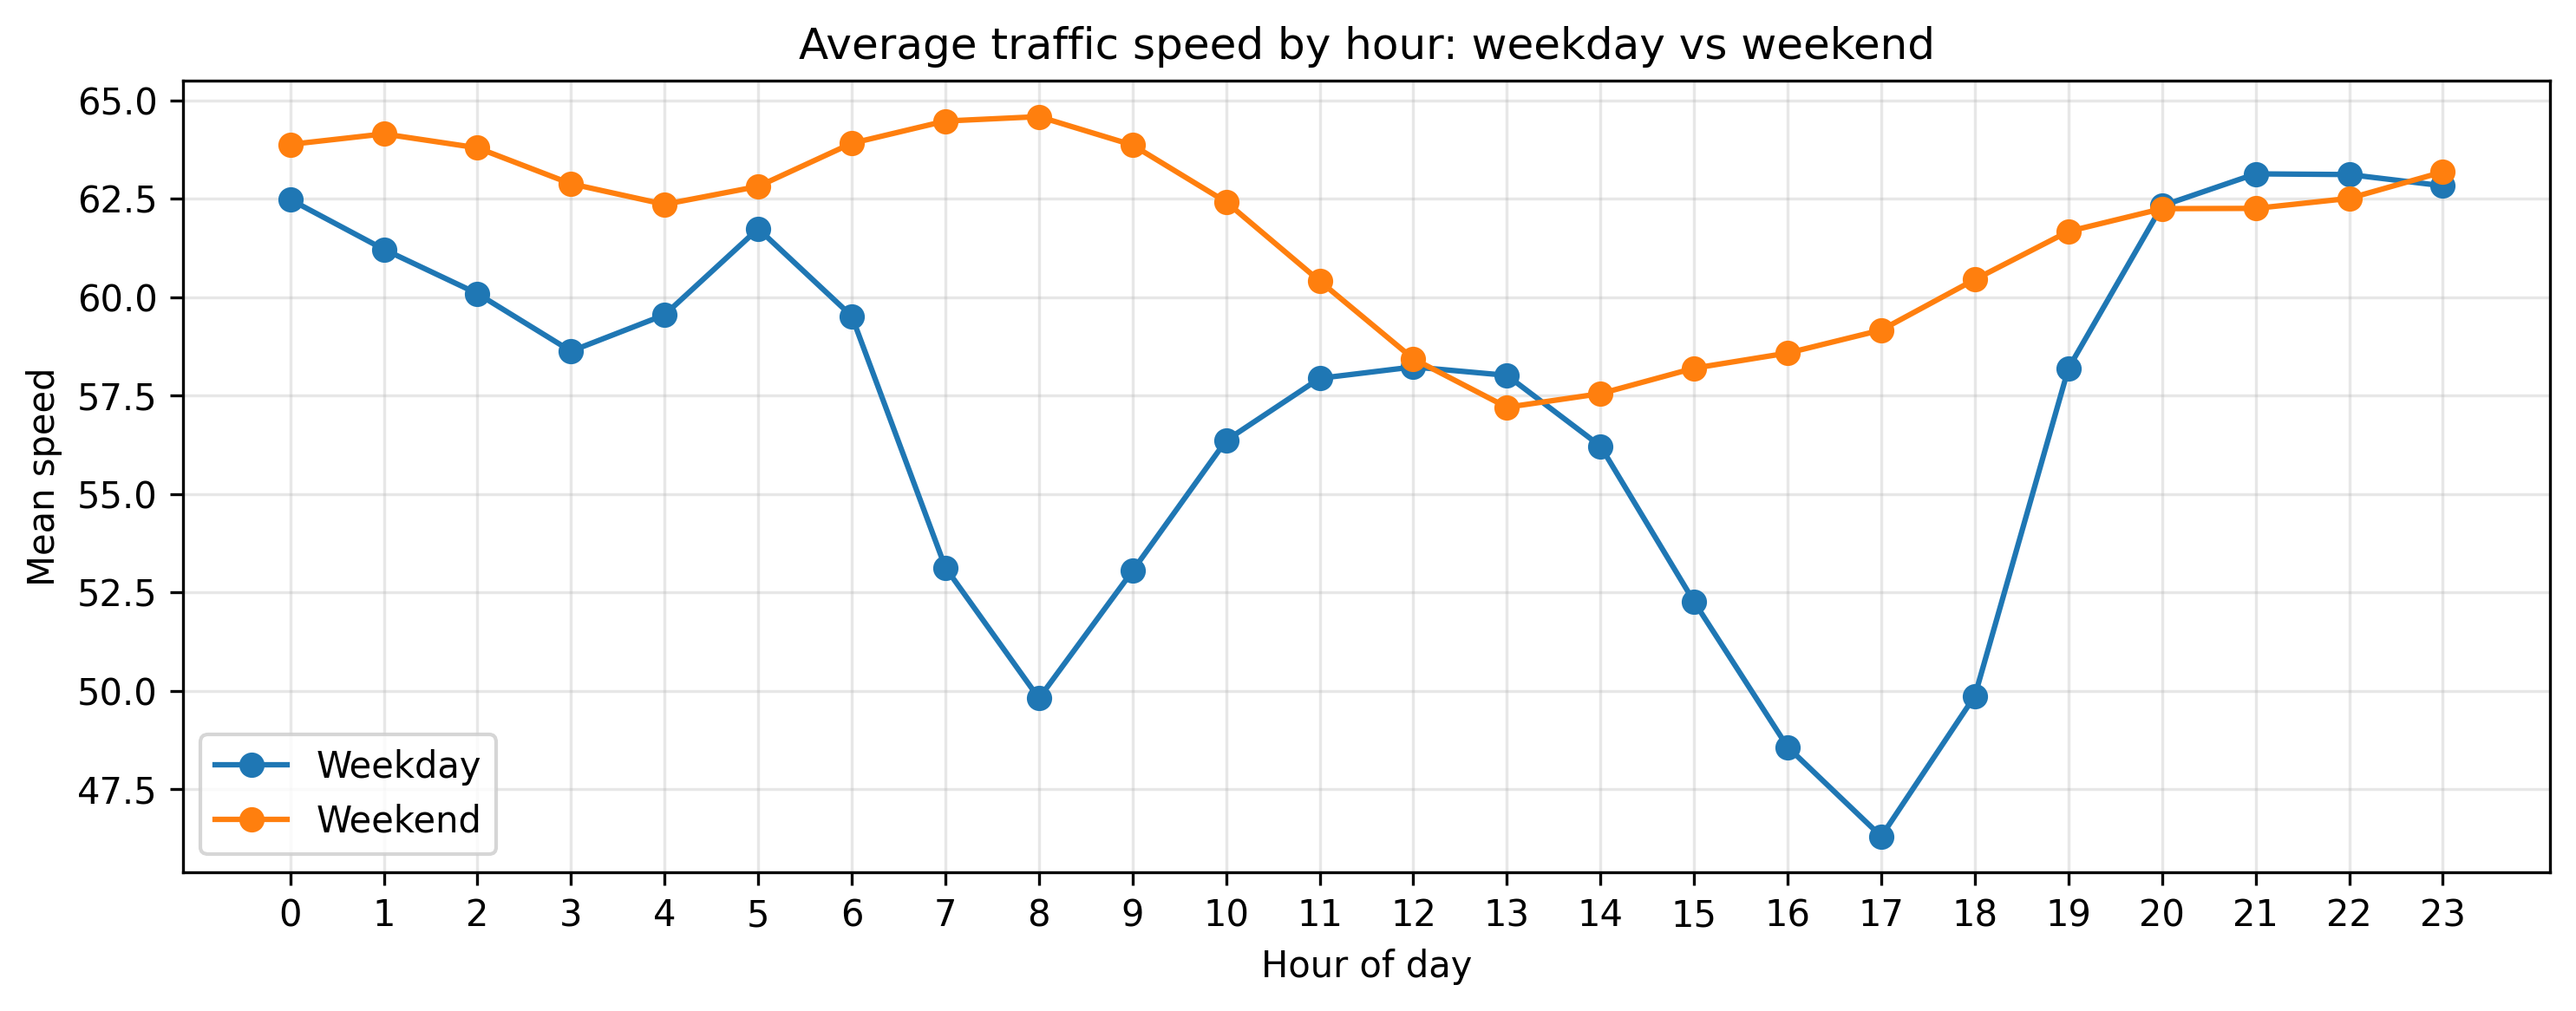
\includegraphics[width=0.75\linewidth]
    {img/data_analysis/weekday_vs_weekend}
    \caption{Average traffic-speed profile by hour of the day, computed
    separately for weekdays and weekends. The different profiles highlight
    both daily and weekly temporal patterns in the METR-LA measurements.}
    \label{fig:temporal_patterns}
\end{figure}

Finally, the distribution of traffic speeds was examined at the individual
sensor level. Considerable heterogeneity was observed across the network, since
the mean traffic speed ranges from approximately 30.89 to 67.73 across
sensors, while the corresponding temporal standard deviations range from
approximately 1.99 to 23.94. Therefore, different sensors exhibit distinct
traffic levels and degrees of variability.

This heterogeneity is particularly relevant for preprocessing, since applying
a single global normalization would ignore the different operating ranges of
individual sensors. For this reason, the normalization strategy described in
Section~\ref{subsec:windowing} estimates separate statistics for each sensor.

Overall, the exploratory analysis identifies two main properties that guide
the preprocessing and modeling choices adopted in this work: a non-negligible
amount of unavailable measurements encoded as zeros, and strong but
heterogeneous temporal traffic patterns across the sensor network.


\subsection{Leakage-Free Data Partitioning}
\label{subsec:splitting}

To preserve the temporal nature of the forecasting problem and prevent
information leakage, the original time series was partitioned
chronologically, without shuffling, into training, validation, and test sets
using a 70\%--10\%--20\% split. Importantly, the partition was performed on
the raw time series before normalization and temporal window construction.

The resulting partitions are summarized in
Table~\ref{tab:chronological_split}. The training set contains 23990
timestamps, followed by 3427 validation timestamps and 6855 test
timestamps. This ordering ensures that validation and test observations
always occur later in time than the observations used for model training.

\begin{table}[t]
    \centering
    \caption{Chronological partition of the original METR-LA time series
    before preprocessing and temporal window construction.}
    \label{tab:chronological_split}
    \begin{tabular}{lrrl}
        \toprule
        Split & Proportion & Timestamps & Time period \\
        \midrule
        Training   & 70\% & 23990 &
        Mar.\ 1 00:00 -- May 23 07:05 \\
        Validation & 10\% & 3427 &
        May 23 07:10 -- Jun.\ 4 04:40 \\
        Test       & 20\% & 6855 &
        Jun.\ 4 04:45 -- Jun.\ 27 23:55 \\
        \bottomrule
    \end{tabular}
\end{table}

All data-dependent preprocessing operations were subsequently fitted using
the training partition only. In particular, the per-sensor normalization
statistics were estimated exclusively from training observations and then
reused unchanged for validation and test data.

Temporal windows were also constructed independently within each partition.
Consequently, an input--target pair can never cross a split boundary. For
example, a training input window cannot use observations from the validation
period as future targets. This procedure preserves the chronological
separation between model development and final evaluation.



\subsection{Missing-Value Handling}
\label{subsec:missing}

Based on the exploratory analysis in
Section~\ref{subsec:eda}, zero-valued traffic measurements were interpreted
as unavailable observations and replaced with missing values before further
processing. Missing values were then handled differently in the input
history and in the forecasting targets, since imputing a target would create
artificial ground-truth values and could bias both training and evaluation.

\paragraph{Input histories.}

Missing observations in the input history were first handled through a
limited interpolation procedure. For each sensor independently, only short
internal gaps of at most three consecutive timestamps were interpolated, and
only when valid observations were available on both sides of the gap. Longer
gaps and missing values at the boundaries of an input window were left
unchanged.

This conservative strategy reduces isolated sensor dropouts while avoiding
the reconstruction of long unavailable periods from potentially unrelated
observations. Before interpolation, missing values accounted for
approximately 7.13\%, 7.00\%, and 12.13\% of the input values in the
training, validation, and test windows, respectively. After short-gap
interpolation, these proportions decreased to approximately 6.85\%, 6.83\%,
and 11.92\%.

Therefore, interpolation only
moderately reduces the overall amount of missing data. This is expected
because the procedure deliberately targets short internal gaps while
preserving longer periods of sensor unavailability.

Input windows for which all sensors were unavailable throughout the complete
history were removed, since they contain no temporal information from which a
forecast can be produced. In contrast, a window was retained when only a
subset of sensors was fully unavailable, because observations from the
remaining sensors may still provide useful information, particularly for the
graph-temporal model.

After this filtering step, residual missing input values were replaced by
zero in the standardized domain. Since normalization is performed separately
for each sensor using training statistics, this value corresponds to the
training mean of that sensor rather than to a physical traffic speed of zero.
An input availability mask was retained to distinguish observed from missing
measurements.

\paragraph{Forecasting targets.}

A stricter policy was adopted for the forecasting targets. Target values were
never interpolated or semantically imputed, since doing so would introduce
synthetic ground truth into the optimization and evaluation procedures.
Instead, a binary target-availability mask was constructed and propagated
throughout the complete pipeline.

Windows with no valid target observations over the complete forecasting
period were removed. Partially observed target windows were retained, while
missing target entries were numerically replaced with finite placeholder
values only to maintain valid tensor representations. These entries were
always excluded from the loss and evaluation metrics through the target
mask and therefore never contributed to model optimization or reported
performance.

After filtering fully unavailable input and target windows, the final dataset
contains 22817 training samples, 3240 validation samples, and 6224 test
samples, as reported in Table~\ref{tab:final_dataset}. Despite the missing
periods identified in the raw data, target availability remains above 94\%
at all evaluated horizons, providing a sufficiently large set of valid
observations for model training and evaluation.

\begin{table}[t]
    \centering
    \caption{Number of temporal samples retained after missing-data
    processing and filtering.}
    \label{tab:final_dataset}
    \begin{tabular}{lr}
        \toprule
        Split & Final samples \\
        \midrule
        Training   & 22817 \\
        Validation & 3240 \\
        Test       & 6224 \\
        \bottomrule
    \end{tabular}
\end{table}

Target availability nevertheless remains high at all evaluated horizons,
ranging from approximately 94\% to 97\% depending on the split and forecast
horizon.


\subsection{Normalization and Temporal Windowing}
\label{subsec:windowing}

As discussed in Section~\ref{subsec:eda}, traffic-speed distributions vary
substantially across sensors. For this reason, the data were standardized
independently for each sensor rather than using global statistics shared
across the complete network.

For each sensor $n$, the mean $\mu_n$ and standard deviation $\sigma_n$ were
estimated exclusively from the valid observations in the training partition.
Each available traffic-speed observation $x_{t,n}$ was then transformed as

\begin{equation}
    \tilde{x}_{t,n}
    =
    \frac{x_{t,n}-\mu_n}{\sigma_n}.
    \label{eq:normalization}
\end{equation}

The same training statistics were subsequently applied without modification
to the validation and test partitions. This prevents information from future
partitions from influencing the preprocessing procedure.

After preprocessing and normalization, each chronological partition was
independently transformed into input--target pairs using a sliding-window
procedure. Given an input-history length $H=12$ and a forecasting window
$F=12$, a sample generated at time $t$ consists of the previous 12 traffic
observations and the following 12 observations to be predicted.

More formally, the input and target windows are defined as

\begin{equation}
    \mathbf{X}_t
    =
    \left[
        \tilde{\mathbf{x}}_{t-H+1},
        \ldots,
        \tilde{\mathbf{x}}_{t}
    \right]
    \in \mathbb{R}^{H \times N},
    \label{eq:input_window}
\end{equation}

and

\begin{equation}
    \mathbf{Y}_t
    =
    \left[
        \tilde{\mathbf{x}}_{t+1},
        \ldots,
        \tilde{\mathbf{x}}_{t+F}
    \right]
    \in \mathbb{R}^{F \times N},
    \label{eq:target_window}
\end{equation}

where $N=207$ is the number of sensors. Since measurements are sampled every
five minutes, both $H=12$ and $F=12$ correspond to one hour of traffic
observations.


Although the models jointly predict all $F=12$ future steps, the main
evaluation is performed at three representative forecasting horizons:
$t+3$, $t+6$, and $t+12$, corresponding respectively to 15, 30, and
60 minutes into the future. This allows performance to be analyzed as the
forecasting task becomes progressively more difficult with increasing
prediction horizon.


The windowing procedure was applied jointly to the traffic values and their
availability masks. Consequently, each input window is associated with an
input mask indicating which historical observations are available, while
each target window is associated with a target mask identifying the entries
that can contribute to the training loss and evaluation metrics.

Partially observed windows are therefore retained whenever useful information
is available, rather than being discarded entirely because of a small number
of missing sensor measurements. As described in
Section~\ref{subsec:missing}, unavailable target entries never contribute to
model optimization or performance evaluation.


The resulting preprocessing pipeline therefore preserves the chronological
structure of the forecasting problem, estimates all data-dependent
transformations exclusively from the training period, and explicitly tracks
unavailable observations through masks. The same processed input--target
windows are used by all forecasting approaches described in the following
section, ensuring that differences in performance are attributable to the
forecasting models rather than to different data-processing procedures.